% First write a small introduction about what is ubuntu like it being the 3rd best operating system in the world etc..
This chapter is intended to provide a small background about Ubuntu. Section \ref{chap:about_ubuntu_why} explains why a user should use Ubuntu since this will define the purpose and reason for a user. Section \ref{chap:about_ubuntu_who} digs a little deeper to describe the people behind Ubuntu. Section \ref{chap:about_ubuntu_release} explains in great detail how the Ubuntu release system works and the difference between different types of Ubuntu releases. This chapter ends with a section dedicated to learning to contributing back to Ubuntu.

\section{Why Ubuntu?} \label{chap:about_ubuntu_why}
% Explain the benefits of using ubuntu like opensource, secure, social, free, multiuser environment, cheap, effective etc...
This is certainly a valid and important question before proceeding to the rest of this manual. Why Ubuntu? Current Ubuntu users would cite various reasons for this from the freedom of choice to it being free. But let's go through the main reasons why you should definitely give Ubuntu a serious try.

\begin{description}
\item [Free] Ubuntu is and will always be free in the future. Ubuntu is developed by people all over the world embracing the principle of Free libre open-source software (FLOSS). This enables new software and updates to be available free of cost since they are written by volunteers and also the employees of Canonical, the parent company of Ubuntu. The code goes through an extensive review before they are uploaded to maintain the quality of the code.

\item [No Viruses] While using Ubuntu, you do not need to worry about installing any anti-virus programs since Ubuntu is completely free of viruses. Any security risks are fixed immediately due to an active community of Ubuntu users. 

\item [Community Support] When you need help using your system, the community is available everywhere around you to support you at all times. All this are done voluntarily by people passionate about Ubuntu. This Ubuntu manual you are reading is a proof of this statement. 

\item [Up to date software] Ubuntu will always be up to date with updates released regularly to ensure that your system is secure and bug free. These regular updates will always be available for free. You will be notified automatically when updates are available.

\item [Beautiful, Polished, Stable] These are the goals of every Ubuntu release. Your Ubuntu is designed with the help of the community and experts after extensive discussion. Ubuntu is regularly user tested to ensure that it is easy and simple to use while preserving its elegance and polish.
\end{description}

\section{Who is behind Ubuntu?} \label{chap:about_ubuntu_who} \index{Mark Shuttleworth}
% List out the founder of Ubuntu, the ubuntu team, community, and its connection to Debian
Ubuntu was founded by Mark Shuttleworth, a South African entrepreneur coming up with their first release Ubuntu 4.10 codenamed Warty Warthog in October 2004. Ubuntu is backed by its parent company Canonical, also created by Mark Shuttleworth. Contributions to Ubuntu are shared by Canonical, other companies and the thousands of volunteers who bring their expertise to develop Ubuntu. Community members start small but gradually get more responsibility by earning the respect of the community. In short, Ubuntu is a community driven open source project. Ubuntu is built on the Debian base which in itself is strongly backed by the community.


\section{Ubuntu Releases} \label{chap:about_ubuntu_release} \index{Ubuntu Release Cycle}
% 6 months cadence, normal releases, LTS, support
Before proceeding to explain about how Ubuntu is released, it would be good to understand the meaning of the word \emph{cadence}.Cadence on its own means balanced and rhythmic flow. What does cadence mean in the world of Ubuntu? Quoting Ubuntu's founder Mark Shuttleworth, "Cadence is about releasing on a predictable rhythm." The Ubuntu team maintain a precise time rhythm in releasing a new version of Ubuntu. They release a new version of Ubuntu every six months. Let's now continue with the different types of Ubuntu releases.\\

\par \noindent As usual there is a new Ubuntu release every six months. However, not everyone would like to upgrade their system every six months. With this in mind, Ubuntu has two types of releases or should we say two versions of a release. There is a so called Long-Term-Support release (LTS) and normal releases. Cadence remains but types do change. Every two years there is a LTS release and in between these two years there are normal releases as usual. So the order of the release would be in the order shown in figure \ref{fig:ubuntu-release-cycle}. \\

\begin{figure}[h]	
	\begin{center}
	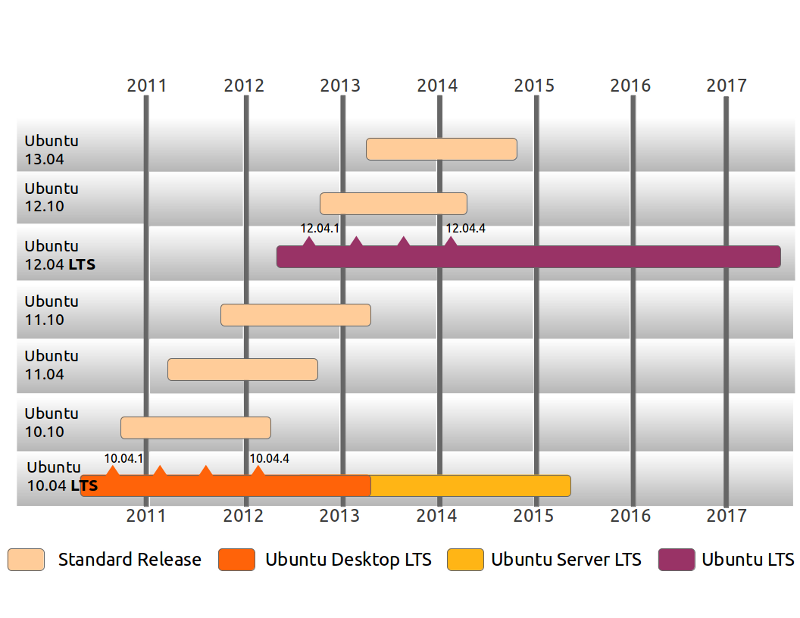
\includegraphics[width=300pt]{./images/about-ubuntu/ubuntu-release-cycle.png}
	\caption{Ubuntu Release Cycle}	
	\label{fig:ubuntu-release-cycle}	
	\end{center}
\end{figure}

\par \noindent Before explaining about the two types of a release, let us make a little digression and compare this with Windows updates since they can be compared easily. When you have a fresh install of Windows on your computer you would have probably noticed that the system is constantly updated to get security patches and bug fixes. These are basically support provided by Microsoft. How long will one version of Windows receive updates depends on how long Microsoft decides to support its development and upgrade. This is similar with Ubuntu and the two mentioned types of a release. Only here Canonical  decides how long an Ubuntu release is supported. \\

\par \noindent Long-Term-Support (LTS) releases of Ubuntu are claimed to be stable versions since they are supported by Canonical for five years. So, you can practically use them on your computer for five years with no worry. After that time, you will no longer receive security updates and installation of a new Ubuntu release is recommended.\\

\par \noindent On the other hand, Normal releases are supported for eighteen months. This type of release is targeted at users who like to constantly update to get the latest features. While LTS releases are targeted at corporations and users who would like to stick to one release for as long as they can while still being supported.\\

\par \noindent To summarize everything mentioned above, you can see the Ubuntu release chart in figure \ref{fig:ubuntu-releases} from the very first start of the Ubuntu project. \\

\begin{figure}[h]	
	\begin{center}
	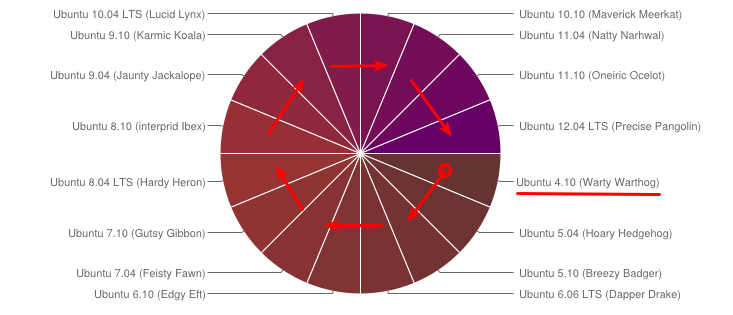
\includegraphics[width=400pt]{./images/about-ubuntu/ubuntu-releases.png}
	\caption{Ubuntu Releases}	
	\label{fig:ubuntu-releases}	
	\end{center}
\end{figure}

\par \noindent Let's explain figure \ref{fig:ubuntu-releases} briefly. The Ubuntu project started in the year 2004. You can see that by looking at the numbers after Ubuntu (e.g. 4.10, 5.04). The first number represents the year while the last two numbers represents the month of a year. Therefore, Ubuntu 4.10 was released in the year 2004 in October, Ubuntu 5.04 is released in the year 2005 in April and so on. \\

\par \noindent You would have also probably noticed that every release has an animal with an agnomen label (hint- Warthy Wartog). These are just code names of a certain release. It's something that Mark Shuttleworth came up with. The name stronly co-relates to the goals of that release. In this case, Ubuntu 12.04 is called Precise Pangolin because the focus of this release is to polish the existing features to precision. For further reading, you are directed to see this youtube video here, where you can actually see what Mark Shuttleworth said about Ubuntu 10.04 Lucid Lynx (\href{http://www.youtube.com/watch?v=l02bhwofEqw}{Ubucon2009}). \index{Ubucon 2009}\\

%\section{Ubuntu derivatives} \label{chap:about_ubuntu_derivatives}

%\par \noindent In chapter \ref{chap:about_ubuntu_who}, you found out that Ubuntu is not a "stand alone" project in the open source world. More precisely, in the world of open source distributions development (hint- Torvalds, other distros, Debian, forks of distros). \\	% Need to be completed

%\par \noindent \textit{This section needs fixing.} These Ubuntu derivatives you can see as  forks, (not something you eat with), of Ubuntu. You can actually connect that with math (derivatives). You derive number and you get some other but the base remains the same. So Ubuntu is the base and other distributions that are derived from it are derivatives. Therefore we have: Xubuntu, Kubuntu, Edubuntu, Goobuntu. Each distro is meant for something else and for some other audience (e.g. Edubuntu is meant for schools and education). 

\section{Contributing to Ubuntu} \label{chap:about_ubuntu_contribute} \index{Contribute}
% Talk about FOSS, anybody can contribute to Ubuntu.....encourage users...the community makes Ubuntu.
If you are new to the open source world, this might be a bit surprising for you. You can actually contribute to the Ubuntu project. Ubuntu development is not done behind closed doors like other operating systems for instance Windows, Unix and Mac OSX. Of course, there are main contributors like the Canonical employees, but as part of the Ubuntu community you can also contribute in certain ways. \\

\par \noindent Certain ways to contribute to Ubuntu are,

\begin{description}

\item [Spread the word about Ubuntu] The easiest and simplest way to contribute to Ubuntu is to let everyone know about Ubuntu. Currently, one of the major stoppers towards widespread use of Ubuntu is the lack of awareness of Ubuntu. You can play an important role in solving this problem by organising Ubuntu release parties or by just word of mouth.

\item [Submit bug reports] While using Ubuntu if you encounter any bug, submit a bug report so that the Ubuntu developers are aware of the issue. All bugs are reported and tracked in \href{https://launchpad.net/}{Launchpad}. It is a bug tracker that aids the software team to collaborate on bug reports and provide fixes. You can submit bug reports via the terminal and the dash (you'll find out about terminal more later by reading this manual). You can read more about this in section \ref{sect:bugreport-terminal}.

\item [Involve yourself in Ubuntu development] After you get more comfortable with Ubuntu, you might have a wish to aid in developing it someday. Ubuntu has many projects like desktop, server, kernel etc. Contributing to Ubuntu development can take place in various levels. You can help by being a translator, programmer or by contributing as graphic designer. The options are endless. You can read more about contributing \href{http://developer.ubuntu.com/}{here} \index{Developer}.

%%Here is also more material for further readings, where you can actually learn about packaging which is very important part of an Ubuntu project. (Packaging tutorial for beginners).
\end{description}

\par \noindent In the open source world you always start as a volunteer. Starting small, you can gradually climb the ladder from being a volunteer to perhaps an Ubuntu Member or a Canonical employee. Linus Torvalds started working on his pet project. This project turned big to be called the Linux kernel which can now be found everywhere from mobiles, computers to small chips. As one of the main Linux kernel maintainers, namely Greg Kroah-Hartman, said: "Once I was doing this for a hobby. Now I don't have a hobby."  \\

\par \noindent Its entirely up to you. It is Free libre open-source software (FLOSS). You can decide if you want to contribute to the open source world and continue the FLOSS philosophy. That means that you can help it grow and develop. You can even fork Ubuntu, change it to your liking and share it with others. With open source you are not tied with licences, patents or any other kind of constrictions. 
